%===============================%
\section{Cylindrical detector system}
%===============================%
A schematic view of the cylindrical detector system (CDS) with the target system is shown in Fig.~\ref{fig:CDS}.
Charged particles generated by the reaction at the target are reconstructed by a cylindrical drift chamber (CDC), which operates in a magnetic field of 0.7~T provided by a solenoid magnet. A cylindrical detector hodoscope (CDH) is used for particle identification and as a charged particle trigger. An inner hodoscope (IH) is installed to enlarge the acceptance for the tracks out of CDH acceptance. The DEF and BPC, which are already described in Sec. 2.6, are located just upstream of the target chamber. A backward proton detector (BPD) is installed to detect backward scattered particles for another experiment

  \begin{figure}[]
   \begin{center}
    \includegraphics[width=\columnwidth]{./fig/cds_v4.eps}
    \caption{Schematic drawing of the CDS with the target system.}
    \label{fig:CDS}
   \end{center}
  \end{figure}  

\subsection{Solenoid magnet}
The spectrometer magnet of the CDS is of a solenoidal type, whose bore diameter is 1.18~m and whose length is 1.17~m with an overall weight of 23 tons. 
The design of the solenoid magnet is shown in Fig.~\ref{fig:solenoid}. It is located on the final focus point of the K1.8BR beam line. The magnet provides a uniform field strength inside the tracking volume ($|z| <$ 420~mm). In the present experiment, it is operated at 0.7 T.

  \begin{figure}[htbp]
   \begin{center}
    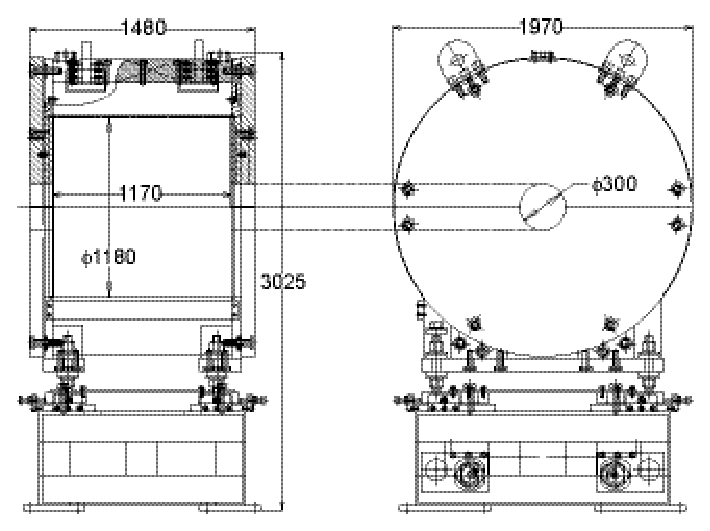
\includegraphics[width=0.8\columnwidth]{ptep/fig/solenoid.eps}
    \caption[Design of the solenoid magnet]{Design of the solenoid magnet (all dimensions in mm).}
    \label{fig:solenoid}
   \end{center}
  \end{figure}  

\subsection{Cylindrical drift chamber}
The CDC is a cylindrical wire drift chamber that contains 15 layers of anode wires. The structure of the CDC is shown in Fig.~\ref{fig:CDC_structure}.
The outer radius is 530~mm and the inner radius is 150~mm, with a total length of 950~mm. The wire length of axial layers is 833.8~mm, thus the angular coverage is 49$^\circ$ $< \theta <$ 131$^\circ$ in the polar angle region corresponding to a solid angle coverage of 66\% of 4$\pi$.
The CDC consists of two aluminum end-plates of 20~mm thickness, a 1~mm thick CFRP cylinder as the inner wall of the CDC, and six aluminum
posts that are placed outside the tracking volume. The CDC uses gold-plated tungsten of 30~$\mu$m$~\phi$ for the sense wires, and gold-plated aluminum of 100~$\mu$m$~\phi$ for the field and guard wires. These wires are supported by feedthroughs with a bushing inserted at the end. Bushes with an 80 and 200 $\mu$m$~\phi$ hole are used for the sense and field/guard wires, respectively.

The CDC has 15 layers of small hexagonal cells with a typical drift length of 9~mm, which are grouped into 7 super-layers as shown in
Fig.~\ref{fig:CDC_cell}. Table~\ref{tab:CDC} gives the detailed parameters of the wire configuration. The layers are in the radial region from 190.5~mm (layer \#1) to 484.5~mm (layer \#15). The 8 stereo layers tilted by about 3.5$^\circ$ are used to obtain longitudinal position information. The number of readout channels is 1816 and the total number of wires in the CDC is 8064.

  \begin{figure}[]
   \begin{center}
    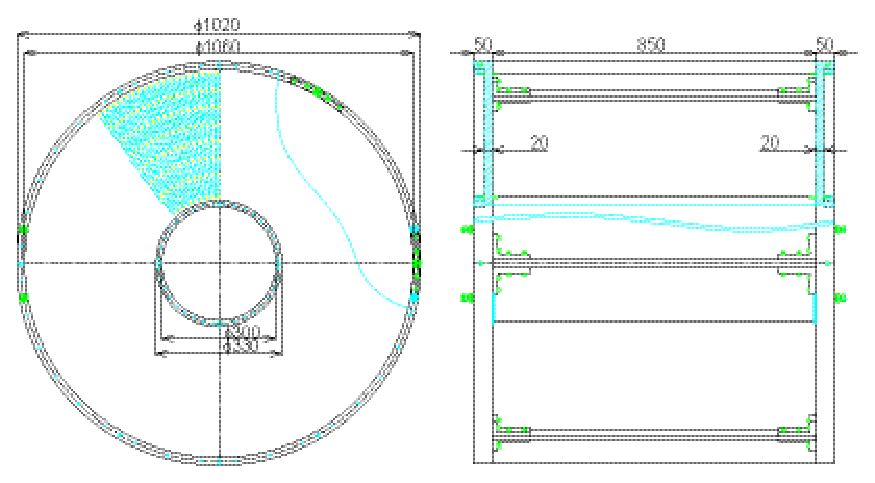
\includegraphics[width=0.8\columnwidth]{ptep/fig/CDC_structure.eps}
    \caption[Design of the CDC.]{Design of the CDC (all dimensions in mm).
    The CDC consists of two aluminum end-plates, a 1~mm thick CFRP
    cylinder as an inner wall, and six aluminum posts that are placed
    outside the tracking volume.}
    \label{fig:CDC_structure}
   \end{center}
  \end{figure}  

  \begin{figure}[]
   \begin{center}
    \includegraphics[width=0.5\columnwidth]{ptep/fig/CDC_cell.eps}
    \caption{Cell structure of the CDC.}
    \label{fig:CDC_cell}
   \end{center}
  \end{figure}  

 \begin{table}[]
  \begin{center}
   \caption{Wire configuration of the CDC.}
   \label{tab:CDC}
   \begin{tabular}{cccccccc}
\hline	\hline														
Super-	&	\multirow{2}{*}{layer}	&	Wire	&	Radius	&	\multicolumn{2}{c}{Cell width}			&	\small{Stereo angle}	&	Signal	\\
layer	&		&	direction	&	(mm)	&	(degree)	&	(mm)	&	(degree)	&	channels	\\
\hline															
\multirow{3}{*}{A1}	&	1	&	$X$	&	190.5	&	\multirow{3}{*}{5.00}	&	16.7	&	0	&	72	\\
	&	2	&	$X'$	&	204	&		&	17.8	&	0	&	72	\\
	&	3	&	$X$	&	217.5	&		&	19	&	0	&	72	\\
\hline															
\multirow{2}{*}{U1}	&	4	&	$U$	&	248.5	&	\multirow{2}{*}{4.00}	&	17.3	&	-3.55	&	90	\\
	&	5	&	$U'$	&	262	&		&	18.3	&	-3.74	&	90	\\
\hline															
\multirow{2}{*}{V1}	&	6	&	$V$	&	293	&	\multirow{2}{*}{3.60}	&	18.4	&	3.77	&	100	\\
	&	7	&	$V'$	&	306.5	&		&	19.3	&	3.94	&	100	\\
\hline															
\multirow{2}{*}{A2}	&	8	&	$X$	&	337.5	&	\multirow{2}{*}{3.00}	&	17.7	&	0	&	120	\\
	&	9	&	$X'$	&	351	&		&	18.4	&	0	&	120	\\
\hline															
\multirow{2}{*}{U2}	&	10	&	$U$	&	382	&	\multirow{2}{*}{2.40}	&	16	&	-3.28	&	150	\\
	&	11	&	$U'$	&	395.5	&		&	16.6	&	-3.39	&	150	\\
\hline															
\multirow{2}{*}{V2}	&	12	&	$V$	&	426.5	&	\multirow{2}{*}{2.25}	&	16.7	&	3.43	&	160	\\
	&	13	&	$V'$	&	440	&		&	17.3	&	3.54	&	160	\\
\hline															
\multirow{2}{*}{A3}	&	14	&	$X$	&	471	&	\multirow{2}{*}{2.00}	&	16.4	&	0	&	180	\\
	&	15	&	$X'$	&	484.5	&		&	16.9	&	0	&	180	\\
\hline\hline
   \end{tabular}
  \end{center}
 \end{table}

The drift gas is 1 atm of mixed argon (50\%)-ethane (50\%). A high voltage is applied to the field and guard wires, and the sense wires are kept at ground potential. For the first super-layer (A1) and the second one (U1), a high voltage of -2.8 kV is applied to the potential wires, and -2.7 kV to the potential wires of the other super-layers. In addition, -1.5 kV, -1.8 kV, and -0.6 kV are applied to the innermost, the outermost, and the other guard wires, respectively.
The readout electronics of the CDC consists of a preamp card with ASDs (SONY-CXA3653Q, $\tau$ = 16~ns), an LVDS-ECL converter, and a TDC --
the same as those for the beam line chambers. 

\subsection{Cylindrical detector hodoscope}
The CDH is a segmented plastic scintillation counter used for the charged
particle trigger and particle identification.
The CDH is located at a radius of 544~mm from the beam axis covering
a polar angle range from 54 to 126 degrees corresponding to a solid
angle coverage of 59\% of 4$\pi$.

The CDH consists of 36 modules, individually mounted on the inner wall
of the solenoid magnet.
The scintillators are made of Eljen EJ-200, with dimensions of 790~mm
in length, 99~mm in width, and 30~mm in thickness.
The scintillation light is transferred through light guides to a pair of
Hamamatsu R7761 fine-mesh 19-dynode photomultipliers 1.5 inches in
diameter.

The CDH is operated in the 0.7~T magnetic field with a typical PMT gain
of $\sim10^6$. 
The measured average time resolution of the CDH without a magnetic field
is 71 $\pm$ 3 ~ps ($\sigma$), obtained with cosmic ray data. 
The error represents the variation among the segments.

\subsection{Inner Hodoscope}
An inner hodoscope (IH) is a segmented plastic scintillation counter mounted on the inner wall of the CFRP cylinder of the CDC at a radius of 140~mm from the beam axis. The IH covers a polar angle range from 27 to 153 degrees corresponding to a solid angle coverage of 89\% of 4$\pi$.

The IH consists of 24 ELJEN EJ-200 scintillators with dimensions of 600~mm in length, 37~mm in width, and 3~mm in thickness. Each segment is overlapped by 1 mm. % as shown in Fig. \ref{fig-IH}. 
Due to the strong magnetic field and a limited space, multi-pixel photon counters (MPPCs) with a 3 mm $\times$ 3 mm sensitive area were used (Hamamatsu S10362-33-100C). The scintillation light is collected by 4 wavelength-shifting fibers embedded in the scintillator and connected to an MPPC with a specially designed connector. The MPPC signal is read out by using a preamplifier (HOSHIN). 

\if0
  \begin{figure}[]
   \begin{center}
    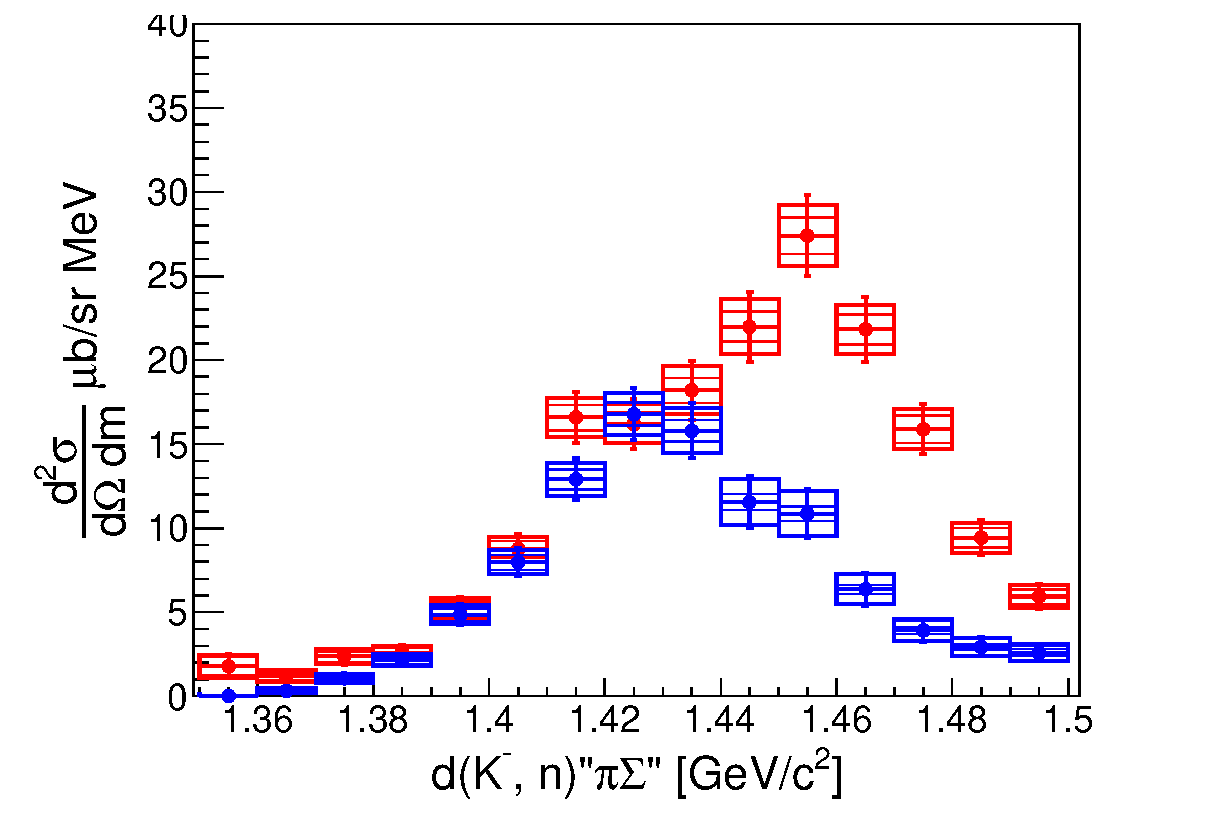
\includegraphics[width=10cm]{fig/tmp.eps}
    \caption{Schematic drawing of the IH.}
    \label{fig-IH}
   \end{center}
  \end{figure}  
\fi  
\subsection{Backward proton detector}
A backward proton detector (BPD) is installed at the most upstream of the CDS to enlarge the acceptance for backward-going charged particles. In particular, it aims to detect a proton from the $\Lambda(1405) \to \Sigma^0\pi^0, \Sigma^0 \to \Lambda\gamma, \Lambda \to p\pi^-$ decay chain in another experiment with the $d(K^-,n)$ reaction (J-PARC E31). 

The BPD is a plastic scintillator hodoscope array with the size of 350 mm (horizontal) $\times$ 340 mm (vertical). It is segmented into 70 units of 5~mm $\times$ 5~mm $\times$ 340~mm scintillation counter made of Eljen EJ-230. Two MPPCs with a 3 mm $\times$ 3 mm sensitive area (Hamamatsu S10362-33-050C) were directly put on both sides of each slab. Signals from the MPPCs are read out by fast timing amps (ORTEC FTA820). 
The BPD is not used in the present analysis except for an energy loss calculation for the kaon beam.
